\chapter{User documentation}
This part of the documentation is focused on the end user. We introduce
installation details and manual for program usage.

\section{Installation guide}
This section documents the process of downloading til running the program.

\subsection{Downloading the code}
The code is available at \url{https://github.com/JankaSvK/thesis}.

\subsection{Hardware requirements}
The software was tested on a system with Intel(R) Core(TM) i5-7300HQ CPU
(2.50GHz, 2496 Mhz, 4Core), 16GB RAM running Microsoft Windows 10 Enterprise.
Minimal requirements are lower, but the copmutation power reflects on frequency
of getting localization results. However, it is multiplatform.

Also two cameras are needed. We tested using a Logitech V-U0018 and Genius
islim 1322AF. A laptop camera may be used too. Requirements for the cameras
are $640\times320$ px resolution and 20 FPS.

\subsection{Dependencies}
Following packages are required to run the application. We also provide
versions of packages used to create and test our implementation.

\begin{center}
\begin{tabular}{l l}
	package	&	version 	\\ \hline
	Python	&	3.4.0 		\\
	NumPy	&	1.13.3 		\\
	OpenCV-contrib	&	3.4.0 	\\ 
	Matplotlib &	2.1.1 		\\
	Tkinter	&	8.6 		\\
	PIL (with ImageTk module)	&	1.1.7 		\\
	dlib	&	19.10.0
\end{tabular}
\end{center}

You can easily check installed versions by running \verb+checkVersions.py+ in
the directory \verb+program/helpers/+.

\section{First run}

In the folder \verb+program/+ we find an entry point for our application
\verb+Main.py+. After starting the application a window will show up (displayed
in figure \ref{fig:application}). With no options provided, the program will
run on the first two cameras available.

\begin{figure}
	\frame{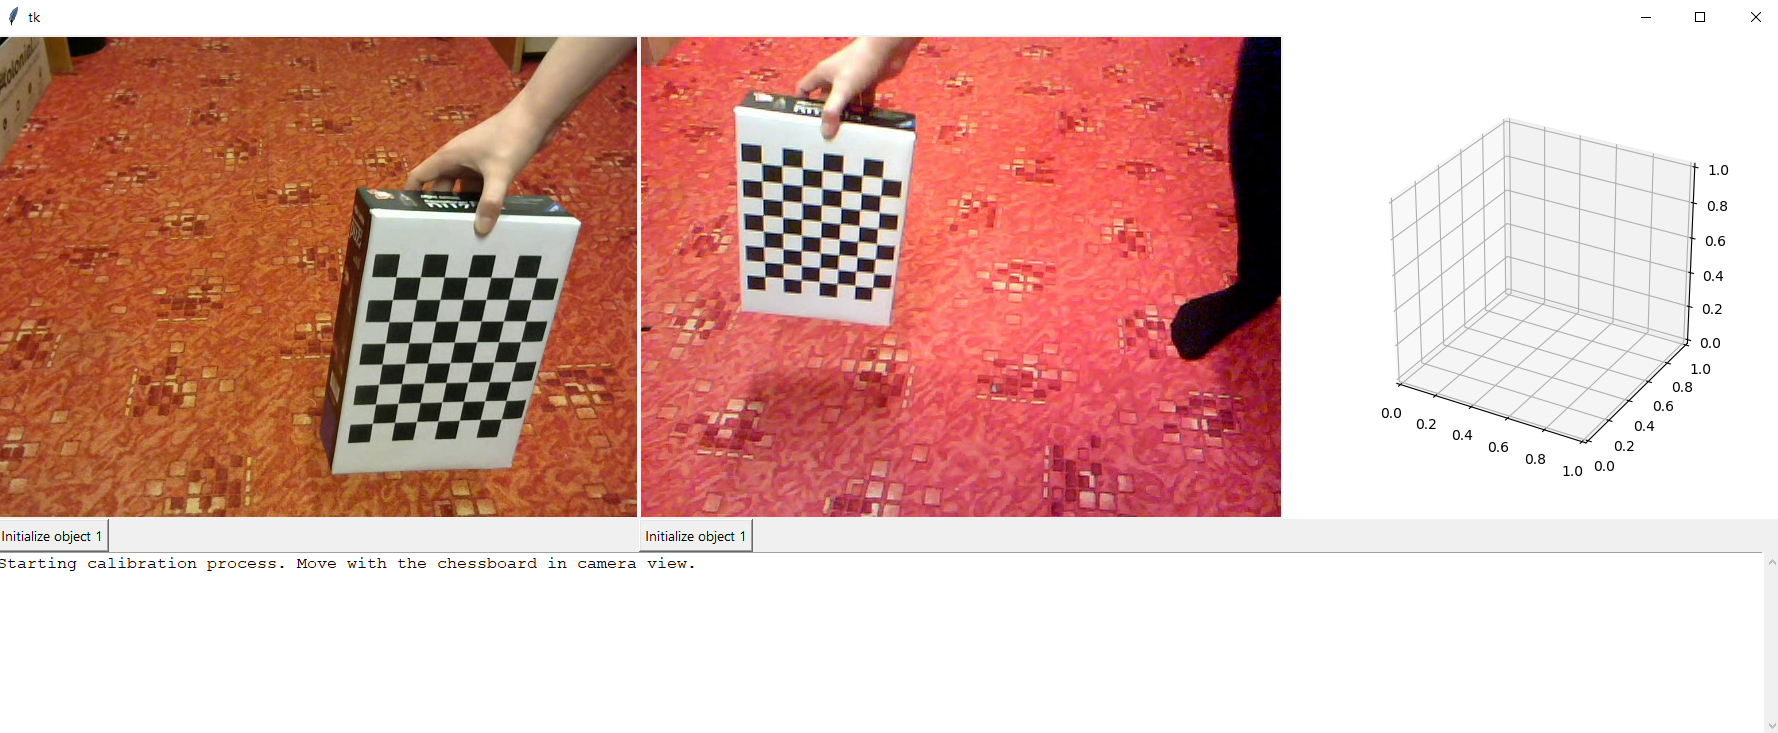
\includegraphics[width=\linewidth]{img/application.png}}
	\label{fig:application}
	\caption{Application window}
\end{figure}

\subsection{Calibration}
As a first step, calibration is expected. We need a calibration pattern --
chessboard, which could be printed. For given chessboard, edit values in
\verb+program/Config.py+. Change the value of \verb+chessboard_inner_corners+
to a number of \emph{inner} corners of your chessboard. Also change
\verb+chessboard_square_size+ to the size of your square in millimiters. It is
important to check, if printed chessboard has squares, not rectangles, since
the printer can slightly scale the image while preprocessing for printing.

For calibration we provide rich set of views of the chessboard. It is important
to move with it, capture it from various angles, distances and in different
parts of the image. Richer set of views increase robustness of the calibration.

After each successful calibration step you will be notified in the console.
After successful stereo calibration, estimated distance between the cameras
will be outputted. If it does not correspond to the reality, consider
recalibration. If it still did not helped, you can increase the number of
images needed for calibration in the config file (be careful, the computation
time may increase).

\subsection{Selecting the objects}
After successful calibration (calibrated with chessboard, or loaded from a
file), we can initialize the trackers. Under each view of the camera, a button
for each object is located.

For a tracker initialization, click on the button. The next two clicks in the
view of the camera, will specify the bounding box for the object. After
initializing trackers in both cameras, localization will automatically start.

If the tracker lost the object, the message will be displayed in the camera
view. Note that, not all trackers are able to recognise losing the object.

\subsection{Localization}
After initialization of the trackers, localization will start automatically.
The results are displayed in the graph on the right. We can rotate graph by
grabbing it by mouse in its window. The dot represents current position and the
line represent the trajectory.

Results from localization are automatically saved.

\section{Additionals}

Different options may be passed to the program (\ref{code:options}). In case no option
is passed program runs on first two available cameras. Firstly calibration for
each camera is done and then stereo calibration. As a tracker is used \verb+KCF+ by default.

\begin{figure}
\lstset{basicstyle=\ttfamily\footnotesize,breaklines=true,frame=lrtb}
\lstinputlisting[label={code:options}, caption={Available options}]{options.txt}
\end{figure}

\subsection{Notes for options}
\emph{Videos} -- Only AVI formats are accepted.

\emph{Trackers} -- As\verb+TRACKER+ may be used a name of implemented tracker. Available trackers
are KCF, MEDIANFLOW, TLD, BOOSTING, MIL, SIMPLEBACKGROUND, HSV,
PATTERNMATCHING, CORRELATION, MOSSE.
\emph{Calibration results} -- Calibration results from previous runs may be
used by specifying path to the file. Take a look on directory hierarchy to know
more.

\subsection{Directory hierarchy}
Results of each calibration and localization are saved.

\subsubsection{Calibration results}
All calibration results are in the directory \verb+program/calib_results+. The
directory has following structure:

\begin{figure}
\dirtree{%
.1 calib{\_}results/.
.2 stereo{\_}calib{\_}results/.
.2 1/.
.2 2/.
 }
 \end{figure}

The results will be automatically saved into corresponding directory. The
naming convention is: \verb+{year}-{month}-{day}-at-{hour}-{minute}.json+,
where the date and time specify the moment when the calibration finished.

\subsection{Localization data}
After closing the program correctly, the data from the object localization will
be saved into \verb+program/localization_data/+. The naming convention for the
file is the same as for the calibration results. However, a suffix is added --
the index of the object.

Saved localization data consist of the four columns separated by tabs. Each
line represents succesful localization. In the first column is the time. In the
rest three columns coordinates are stored (x, y, z).

\subsection{Capturing the videos} 

Capturing and saving videos provide additional program located in
\verb+program/helpers/video_capture.py+. It will automatically capture video
from all available cameras and save it into \verb+captured_videos+. The
capturing can be exited by pressing the key "q".
